\documentclass[a4paper, 12pt]{article}

% ~~~~~~~~~~~~~~~~~~~~~~~~~~~~~~~~~~~~~~~~
% ~~~~~~~~~~~~~~~ PACKAGES ~~~~~~~~~~~~~~~
% ~~~~~~~~~~~~~~~~~~~~~~~~~~~~~~~~~~~~~~~~

\usepackage{tikz}
\usepackage{xcolor}
\usetikzlibrary{arrows}
\usetikzlibrary{positioning}

% ~~~~~~~~~~~~~~~~~~~~~~~~~~~~~~~~~~~~~~~~
% ~~~~~~~~~~~~~~~ PREAMBLE ~~~~~~~~~~~~~~~
% ~~~~~~~~~~~~~~~~~~~~~~~~~~~~~~~~~~~~~~~~

\pagenumbering{gobble}

% ~~~~~~~~~~~~~~~~~~~~~~~~~~~~~~~~~~~~
% ~~~~~~~~~~~~~~~ BODY ~~~~~~~~~~~~~~~
% ~~~~~~~~~~~~~~~~~~~~~~~~~~~~~~~~~~~~

\begin{document}
	\begin{center}
		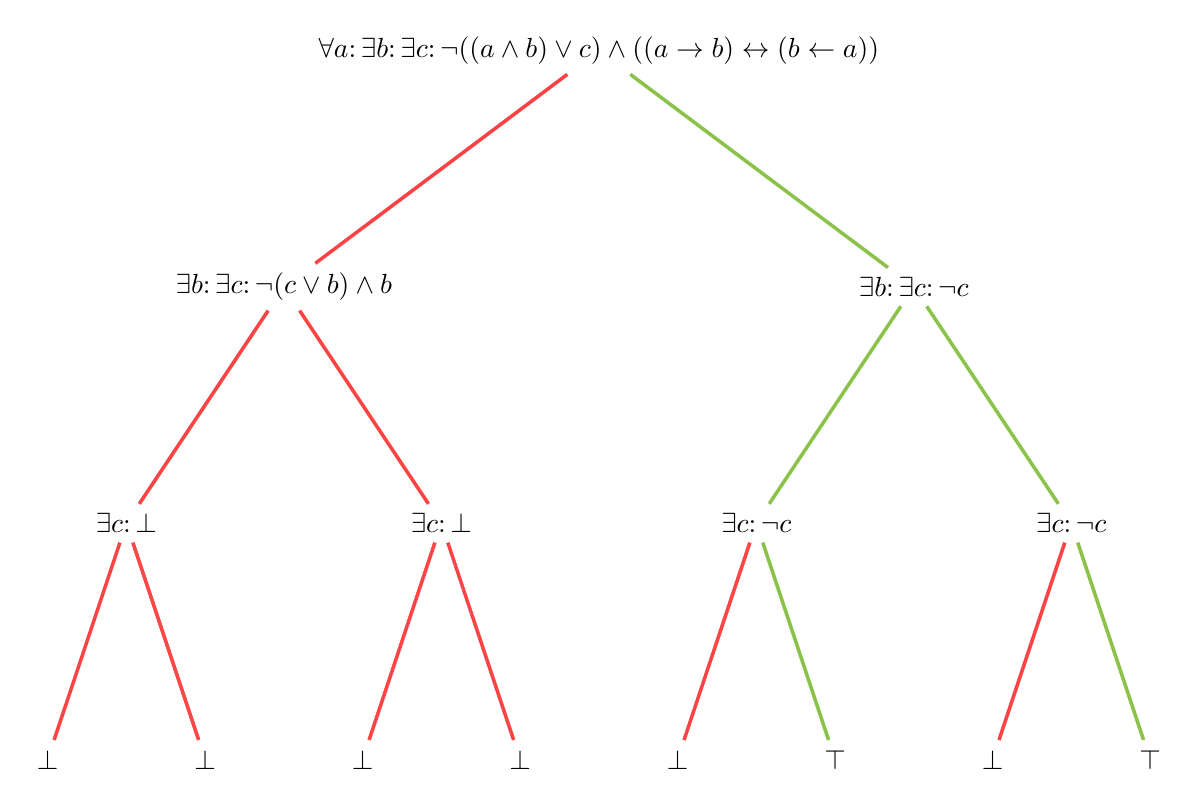
\begin{tikzpicture}[draw]
			\definecolor{RED}{RGB}{252, 68, 68}
			\definecolor{GREEN}{RGB}{139, 195, 74}
			\node[] (147694041372) at ( 0.000,  0.000) {$\forall a\colon \exists b\colon \exists c\colon \neg{((a \land b) \lor c)} \land ((a \rightarrow b) \leftrightarrow (b \leftarrow a))$};
			\node[] (147694041480) at (-4.000, -3.000) {$\exists b\colon \exists c\colon \neg{(c \lor b)} \land b$};
			\node[] (147694041426) at (-6.000, -6.000) {$\exists c\colon \bot$};
			\node[] (147694043549) at (-7.000, -9.000) {$\bot$};
			\node[] (147694043411) at (-5.000, -9.000) {$\bot$};
			\node[] (147694043510) at (-2.000, -6.000) {$\exists c\colon \bot$};
			\node[] (147694043582) at (-3.000, -9.000) {$\bot$};
			\node[] (147694043516) at (-1.000, -9.000) {$\bot$};
			\node[] (147694047097) at ( 4.000, -3.000) {$\exists b\colon \exists c\colon \neg{c}$};
			\node[] (147694047187) at ( 2.000, -6.000) {$\exists c\colon \neg{c}$};
			\node[] (147694047040) at ( 1.000, -9.000) {$\bot$};
			\node[] (147694046983) at ( 3.000, -9.000) {$\top$};
			\node[] (147694047184) at ( 6.000, -6.000) {$\exists c\colon \neg{c}$};
			\node[] (147694047169) at ( 5.000, -9.000) {$\bot$};
			\node[] (147694047181) at ( 7.000, -9.000) {$\top$};
			\draw[-, draw, line width={0.45mm}, color={RED!100}] (147694041372) to (147694041480);;
			\draw[-, draw, line width={0.45mm}, color={RED!100}] (147694041480) to (147694041426);;
			\draw[-, draw, line width={0.45mm}, color={RED!100}] (147694041426) to (147694043549);;
			\draw[-, draw, line width={0.45mm}, color={RED!100}] (147694041426) to (147694043411);;
			\draw[-, draw, line width={0.45mm}, color={RED!100}] (147694041480) to (147694043510);;
			\draw[-, draw, line width={0.45mm}, color={RED!100}] (147694043510) to (147694043582);;
			\draw[-, draw, line width={0.45mm}, color={RED!100}] (147694043510) to (147694043516);;
			\draw[-, draw, line width={0.45mm}, color={GREEN!100}] (147694041372) to (147694047097);;
			\draw[-, draw, line width={0.45mm}, color={GREEN!100}] (147694047097) to (147694047187);;
			\draw[-, draw, line width={0.45mm}, color={RED!100}] (147694047187) to (147694047040);;
			\draw[-, draw, line width={0.45mm}, color={GREEN!100}] (147694047187) to (147694046983);;
			\draw[-, draw, line width={0.45mm}, color={GREEN!100}] (147694047097) to (147694047184);;
			\draw[-, draw, line width={0.45mm}, color={RED!100}] (147694047184) to (147694047169);;
			\draw[-, draw, line width={0.45mm}, color={GREEN!100}] (147694047184) to (147694047181);
		\end{tikzpicture}
		
	\end{center}
	
\end{document}